

\chapter{Pr\'{e}sentation de mon environnement \`{a} SAP}


\section{Présentation de l'équipe}




\begin{figure}[h!]
  \centering
      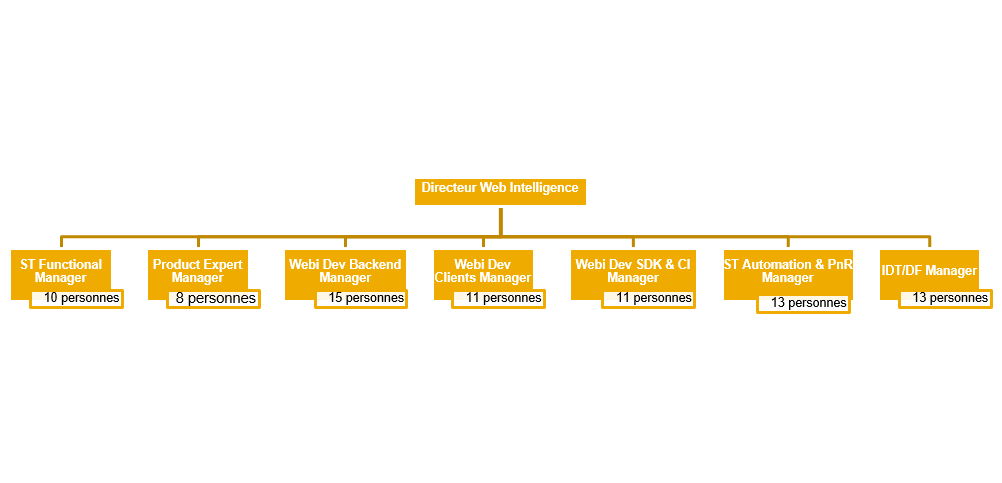
\includegraphics[width=1.2\textwidth]{images/allRaphaelTeam.png}
  \caption{\'{E}quipe de Rapha\"{e}l GEOFFROY - 1}
	\label{figure:}
\end{figure}


\begin{figure}[h!]
  \centering
      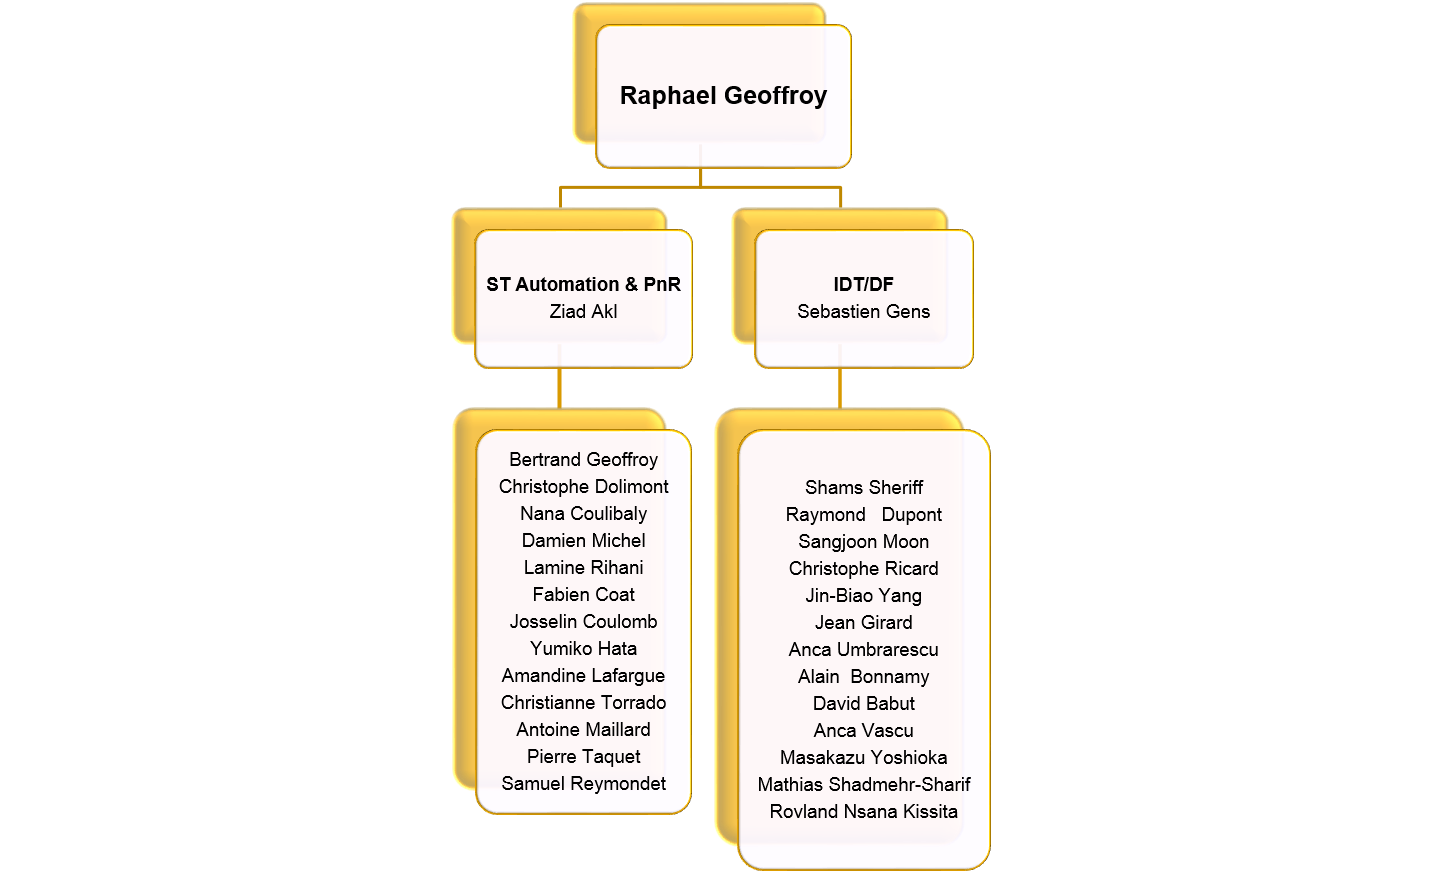
\includegraphics[width=1.2\textwidth]{images/allRaphaelTeam2.png}
  \caption{\'{E}quipe de Rapha\"{e}l GEOFFROY - 2}
	\label{figure:allRaphaelTeam2}
\end{figure}


\begin{figure}[h!]
  \centering
      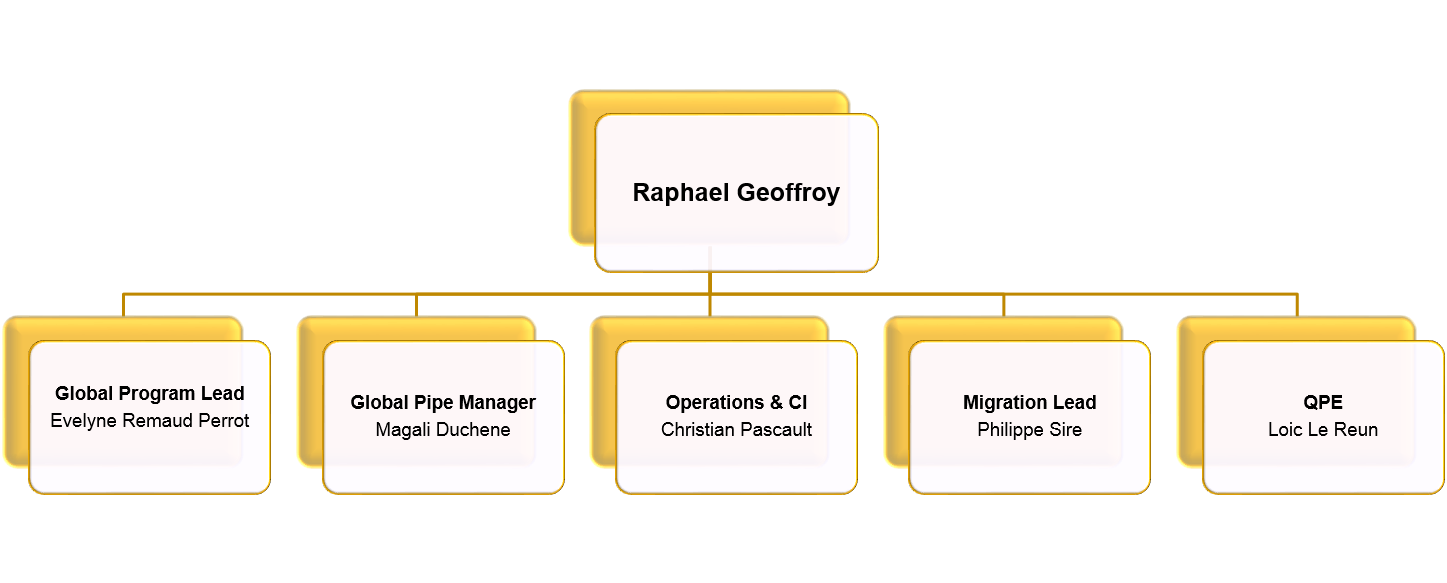
\includegraphics[width=1.1\textwidth]{images/allRaphaelTeam3.png}
  \caption{\'{E}quipe des ind\'{e}pendants de Rapha\"{e}l GEOFFROY}
	\label{figure:}
\end{figure}


\begin{figure}[h!]
  \centering
      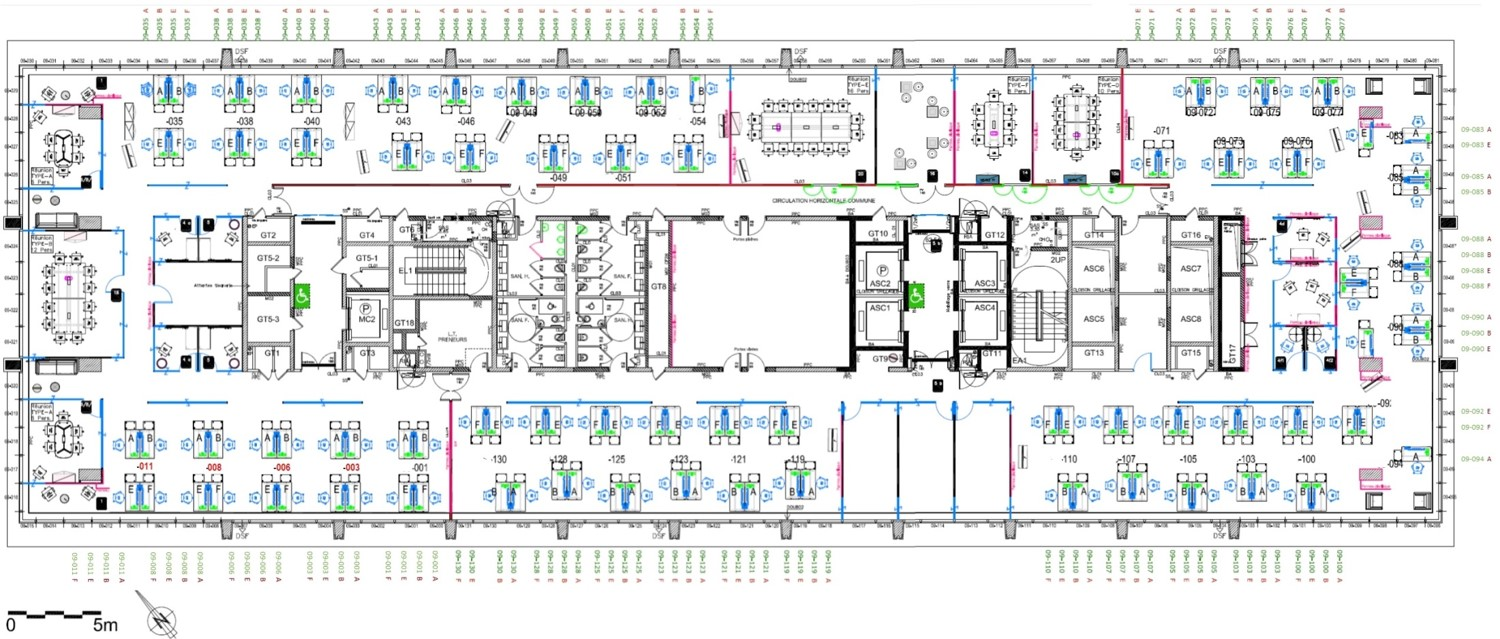
\includegraphics[width=1.2\textwidth]{images/8floor.jpg}
  \caption{8\up{\`{e}me \'{e}tage de la tour SAP \`{a} Levallois-Perret}}
	\label{figure:}
\end{figure}

\begin{figure}[!h]
  \centering
      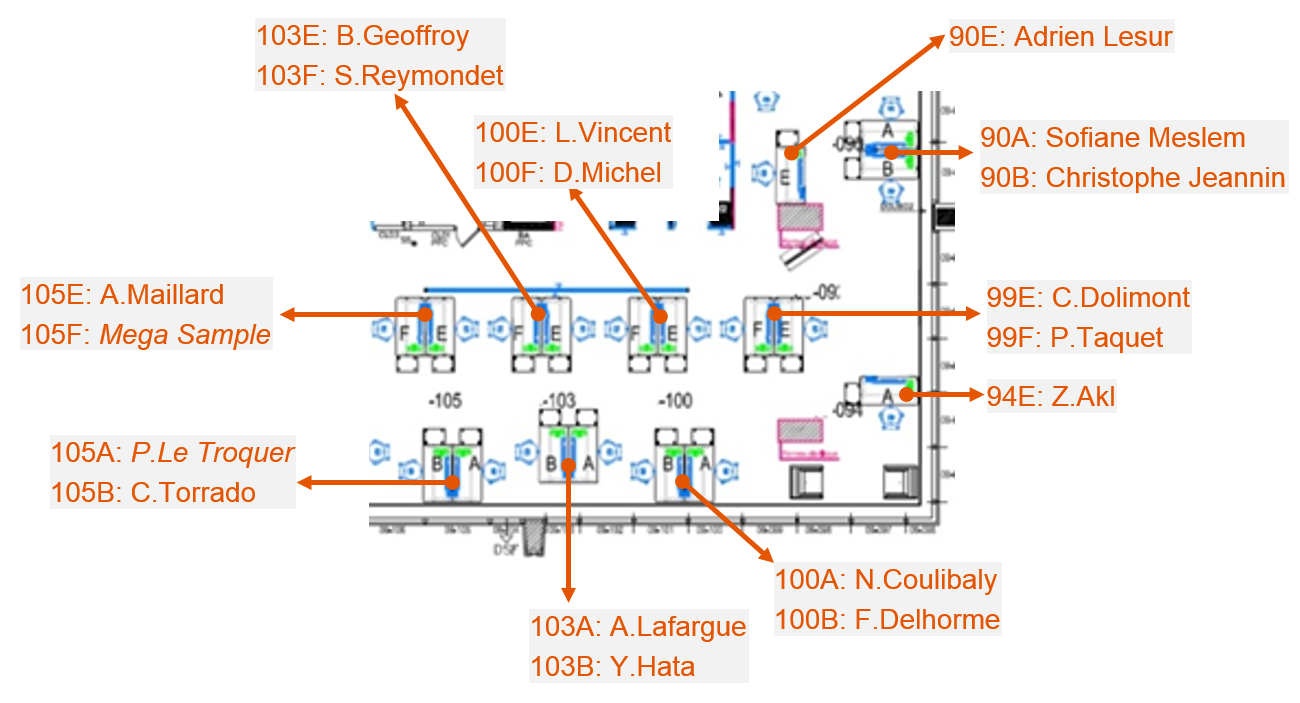
\includegraphics[width=1.2\textwidth]{images/positionnement1.png}
  \caption{8\`{e}me \'{e}tage de la tour SAP \`{a} Levallois-Perret - \'{E}quipe ST Automation - 1}
	\label{figure:}
\end{figure}


\begin{figure}[!h]
  \centering
      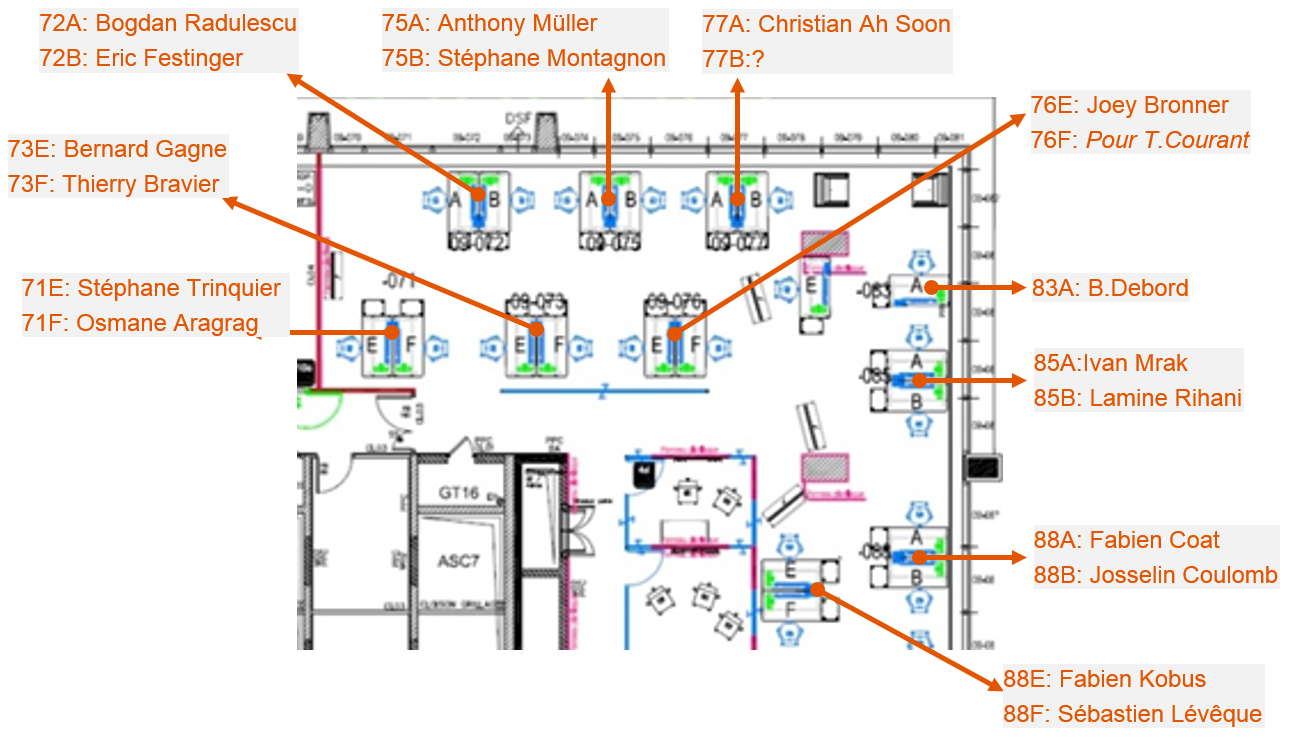
\includegraphics[width=1.2\textwidth]{images/positionnement2.png}
  \caption{8\`{e}me \'{e}tage de la tour SAP \`{a} Levallois-Perret - \'{E}quipe ST Automation - 2}
	\label{figure:}
\end{figure}

\section{Son histoire}
Initialement Rapha\"{e}l GEOFFROY est le chef de toutes les \'{e}quipes de test (QPA-QPE, fonctionnels, performance, automatique, ...). Mais, au moment de la 4.1 SP6, il est devenu le manager du groupe WebI et, parall\`{e}lement, les \'{e}quipes de tests devenaient de plus en plus nombreuses. Ne pouvant plus manager les \'{e}quipes de test, celle-ci ont \'{e}t\'{e} divis\'{e}es en deux cat\'{e}gories principales\footnote{voir illustration \pageref{figure:allRaphaelTeam2} page \pageref{figure:allRaphaelTeam2}} et sont \`{a} la charge de plusieurs managers. D'un c\^{o}t\'{e}, il y a les tests fonctionnels et les tests effectu\'{e}s \textquote{\`{a} la main}, de l'autre, il y a les \textquote{autres}. Autrement dit les tests automatiques, les web services, les performances et les projets en avance sur le reste.\\

L'\'{e}quipe dans laquelle j'ai \'{e}t\'{e} int\'{e}gr\'{e} est \textquote{ST automation \& PnR} ou \textquote{P\&I BIT BI Suite Paris ST Transversal team}\footnote{Product and Innovation BIT Business Intelligence Suite Paris Software Tester Transversal Team}. Elle a \'{e}t\'{e} cr\'{e}\'{e}e en juin 2014, un peu plus d'un mois avant mon arriv\'{e}e.

\section{Sa mission}

L'\'{e}quipe transverse est apparue en réponse aux initiatives qualité, principalement \textquote{un bug - un test}, et à la réorganisation des équipes de test.\\
Particuli\`{e}rement foculis\'{e}e sur le test coverage\index{Test coverage}, différentes missions ce l'\'{e}quipe transverse peuvent être divisées en cinq catégories\footnote{se reporter à l'organigramme page \pageref{pdf:org}} :\\

\begin{description}
	\item[Tests fonctionnels] Ceux-ci sont implémentés par Josselin, Lamine et Fabien. Leurs tests portent sur le SDK de Web Intelligence. 
	\item[Tests automation] Cette partie est assurée par Damien, Christian et Nana. Leur mission est d'ajouter les tests implémentés et de les mettre en production, quelque soit le test (son Framework ou le langage utilisé).
	\item[Benchmark] Assuré par Bertrand, Yumiko et Amandine, ils s'occupent des tests de benchmark, autrement dit, les tests de performance, de stabilité et de scalabilité. Ils sont parfois appelés à implémenter quelques codes mais utilises, en règle général, des logiciels pour générer des charges, ouvrir de multiples documents, installer le produit, répéter la même action des centaines de fois, \ldots. Ils sont aussi en charge des acceptances, autrement dit la validation de tous les tests existants afin de certifier que le produits et fonctionnel.
	\item[Mise en production] Gérée par Christianne. Sa mission est de mettre en production les produits de SAP pour les équipes SAP.
	\item[Développement] Antoine est focalisé sur le développement d'outils internes et sur la construction de rapport WebI.
\end{description}





\section{Ing\'{e}nieur logiciel \`{a} SAP}


Chaque ing\'{e}nieur se voit attribuer un poste de travail (PC et/ou laptop, bureau, \ldots) et un identifiant, le mien \'{e}tant I310911, lui permettant de se connecter sur le portail interne \`{a} SAP ainsi que sur les diff\'{e}rents outils.

 - perforce
- jenkins astec

!!  ici les outils utilis\'{e}s par les employ\'{e}s SAP   !!!
portal : jam, wiki
Les tickets : IT ticket, hrTicket, Ticket CSS

